%%%%%%%%%%%%%%%%%%%%%%%%%%%%%%%%%%%%%%%%%%%%%%%%%%%%%%%%%%%%%%%%%%%%%%%
%%%%  Load the document class and packages                         %%%%
%%%%%%%%%%%%%%%%%%%%%%%%%%%%%%%%%%%%%%%%%%%%%%%%%%%%%%%%%%%%%%%%%%%%%%%
\documentclass[a4paper]{report}
\usepackage{epsfig}            % to insert PostScript figures
\graphicspath{ 
	{./figures/} 
}

%Change figure names
\renewcommand{\figurename}{Fig}

\usepackage[bf,footnotesize]{caption} % make captions small and label bold

\addtocounter{chapter}{1} %Because starting at zero is silly
\makeatletter
\renewcommand{\thesection}{\@arabic\c@section}
\renewcommand{\thefigure}{\@arabic\c@figure}
\makeatother

\usepackage[a4paper,margin=3.7cm,tmargin=2.5cm,bmargin=2.5cm]{geometry} 
\usepackage{textcomp}          % To make nice degree symbols and others\usepackage[bf,footnotesize]{caption} % make captions small and label bold
\usepackage{wrapfig}
%to produce the clickable references along the left in Acroread. This
%package must be included last. 
\usepackage[ps2pdf,bookmarks=TRUE]{hyperref} 

%%%%%%%%%%%%%%%%%%%%%%%%%%%%%%%%%%%%%%%%%%%%%%%%%%%%%%%%%%%%%%%%%%%%%%%
%%%%  Hypertext references for Acrobat                             %%%%
%%%%%%%%%%%%%%%%%%%%%%%%%%%%%%%%%%%%%%%%%%%%%%%%%%%%%%%%%%%%%%%%%%%%%%%
\hypersetup{
	pdfauthor = {SWC},
	pdftitle = {Optics Exercises},
	pdfkeywords = {optics, lenses, refraction, reflection, dispersion,
		telescope, microscope},
	pdfcreator = {LaTeX with hyperref},
	pdfproducer = {dvips + ps2pdf}
}

%%%%%%%%%%%%%%%%%%%%%%%%%%%%%%%%%%%%%%%%%%%%%%%%%%%%%%%%%%%%%%%%%%%%%%%
%%%%  Main text                                                    %%%%
%%%%%%%%%%%%%%%%%%%%%%%%%%%%%%%%%%%%%%%%%%%%%%%%%%%%%%%%%%%%%%%%%%%%%%%
\begin{document}
	
	%set the number of sectioning levels 
	\setcounter{secnumdepth}{2}
	
	\begin{center}
		\textbf{\Large{Assembly Hints}}
	\end{center}
	
	You will be setting up simple optical systems (lenses, light sources, targets, etc) on an optical rail. 
	Here are a few pointers to get you started on the right path.
	

	%%%%%%%%%%%%%%%%%%%%%%%%%%%%%%%%%%%%%%%%%%%%%%%%%%%%%%%%%%%%%%%%%%%%%%%
	\section{General comments on Thorlabs parts}
	%%%%%%%%%%%%%%%%%%%%%%%%%%%%%%%%%%%%%%%%%%%%%%%%%%%%%%%%%%%%%%%%%%%%%%%
	
	\begin{itemize}
		\item \textbf{Do not} touch lens surfaces. Hold lenses by the rim or use lens paper.
		\item \textbf{Do not} touch the coated surface of mirrors or optical filters. These are very hard to clean without smearing/scratching, and they are expensive.
		\item \textbf{Do not} force parts together. All parts should screw together or fit together easily.
		\item \textbf{Do not} over-tighten screws. Gentle pressure with a long-handled Allen key is sufficient. 
		\item Shit happens! If you loose or damage any parts please let the organisers know so the kits stay in good shape.
	\end{itemize}
	
	%%%%%%%%%%%%%%%%%%%%%%%%%%%%%%%%%%%%%%%%%%%%%%%%%%%%%%%%%%%%%%%%%%%%%%%
	\section{Basic assembly guide}
	%%%%%%%%%%%%%%%%%%%%%%%%%%%%%%%%%%%%%%%%%%%%%%%%%%%%%%%%%%%%%%%%%%%%%%%
	
	\begin{itemize}
	\item The black post holders (Fig.~\ref{fig:post}) are screwed to rail carriages that can be mounted on the long rail.
	\item Posts bearing an optical device are inserted into the post holders. 
	\item Use short screws to secure the post holder to the carriage. 
	\item Clamp the rail to the table.
	\item  Make sure all the rail carriages face the same way; otherwise they are not centered with respect to each other (screws on the same side).
	\item The red `lens ring tool' is used to secure lenses to lens holders using threaded lens rings. 
	\end{itemize}
	
	\begin{figure}[h]
		\center
		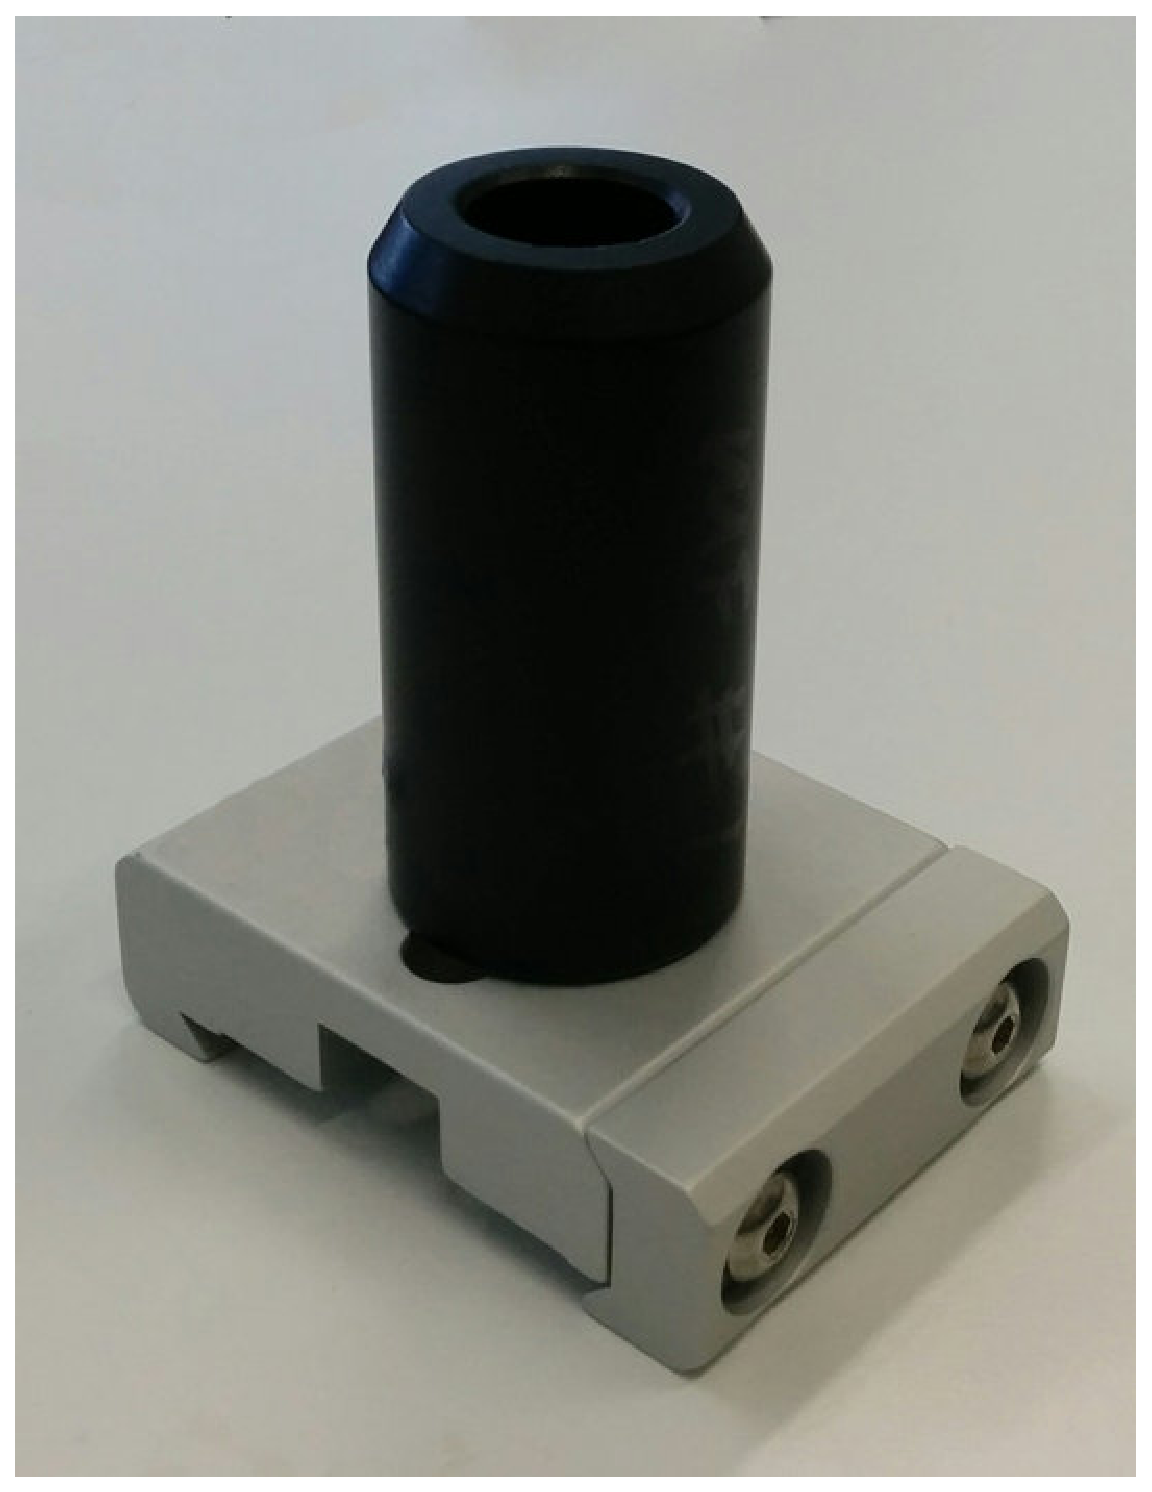
\includegraphics[width=0.9in]{post_mounted.eps}
		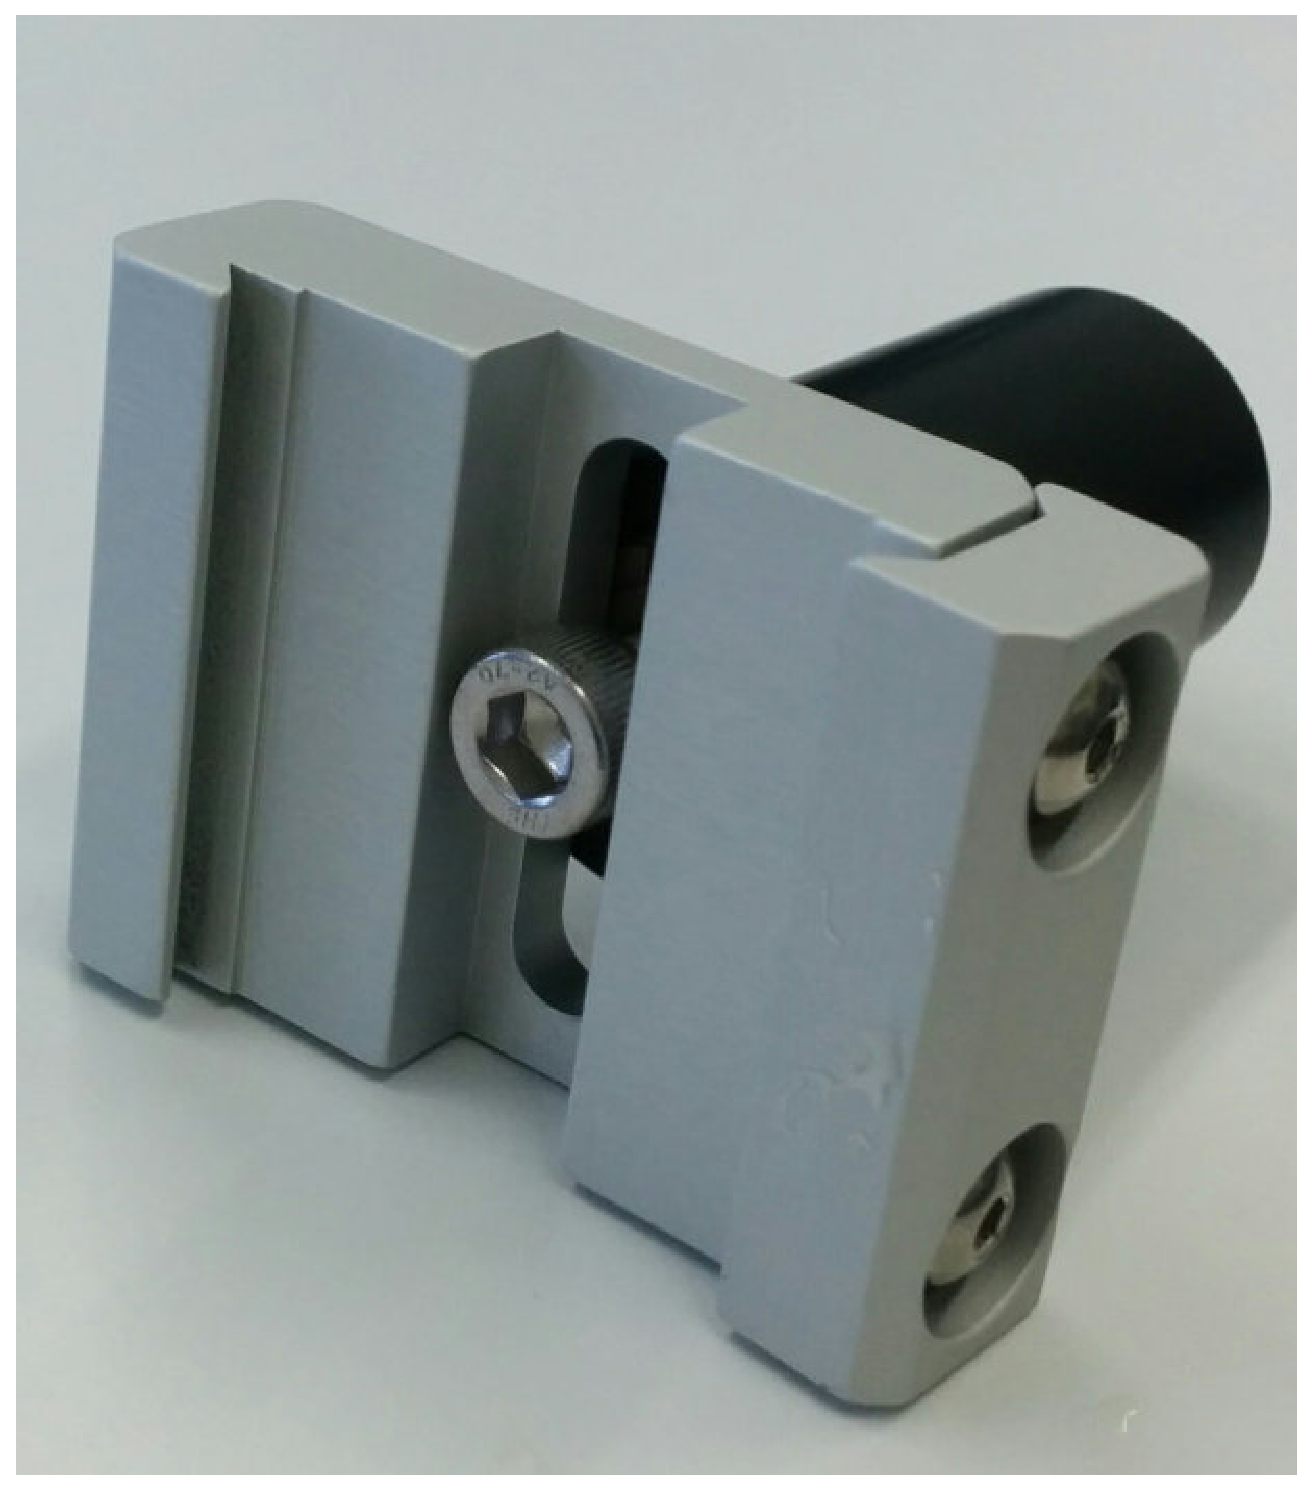
\includegraphics[width=1.03in]{post_mounted_underside.eps}
		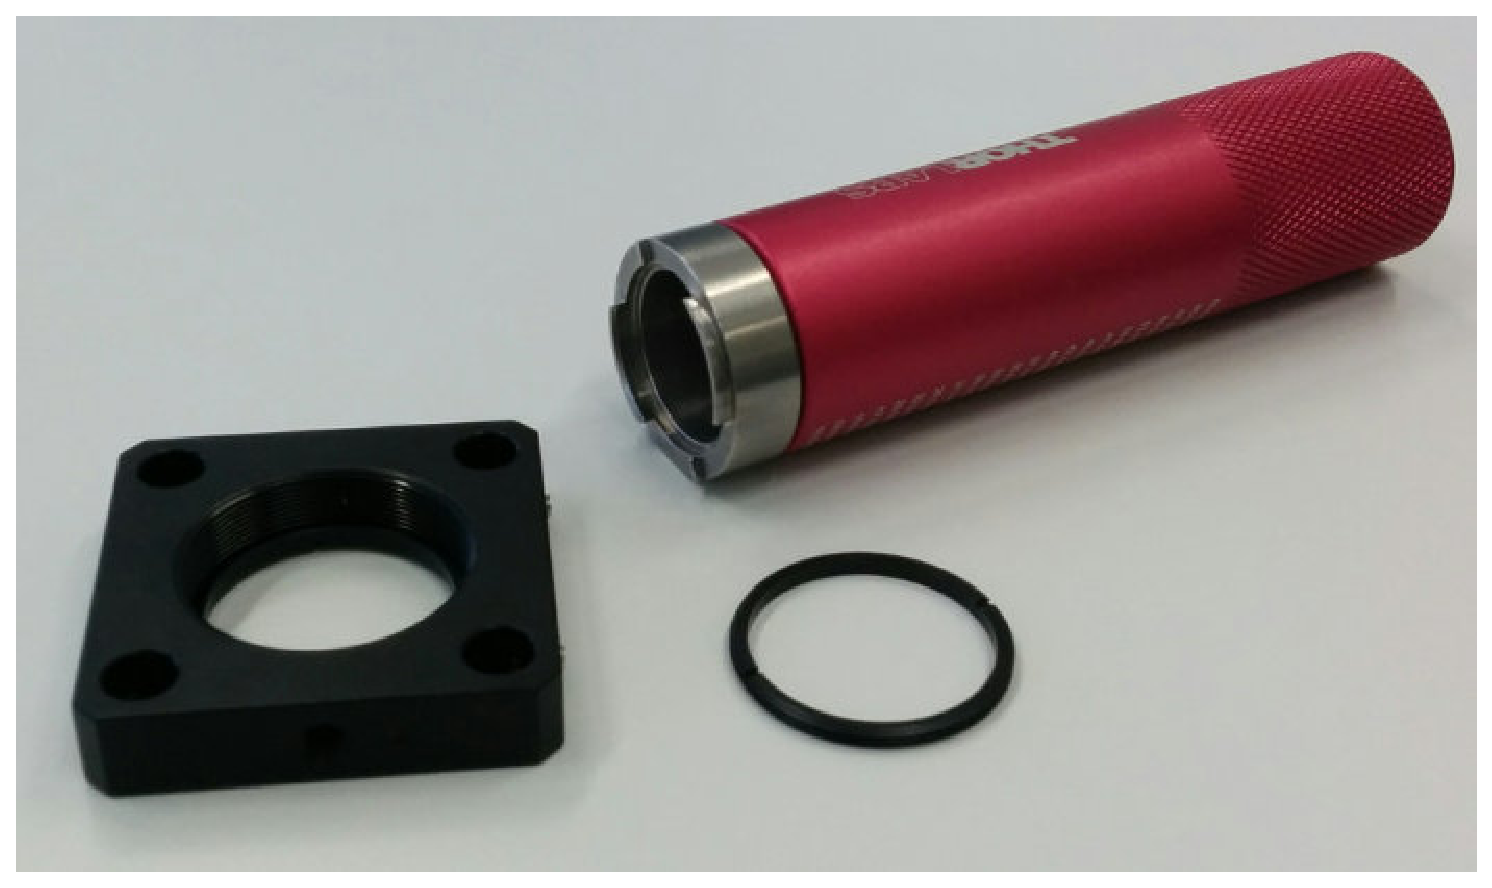
\includegraphics[width=2in]{lens_tool.eps}
		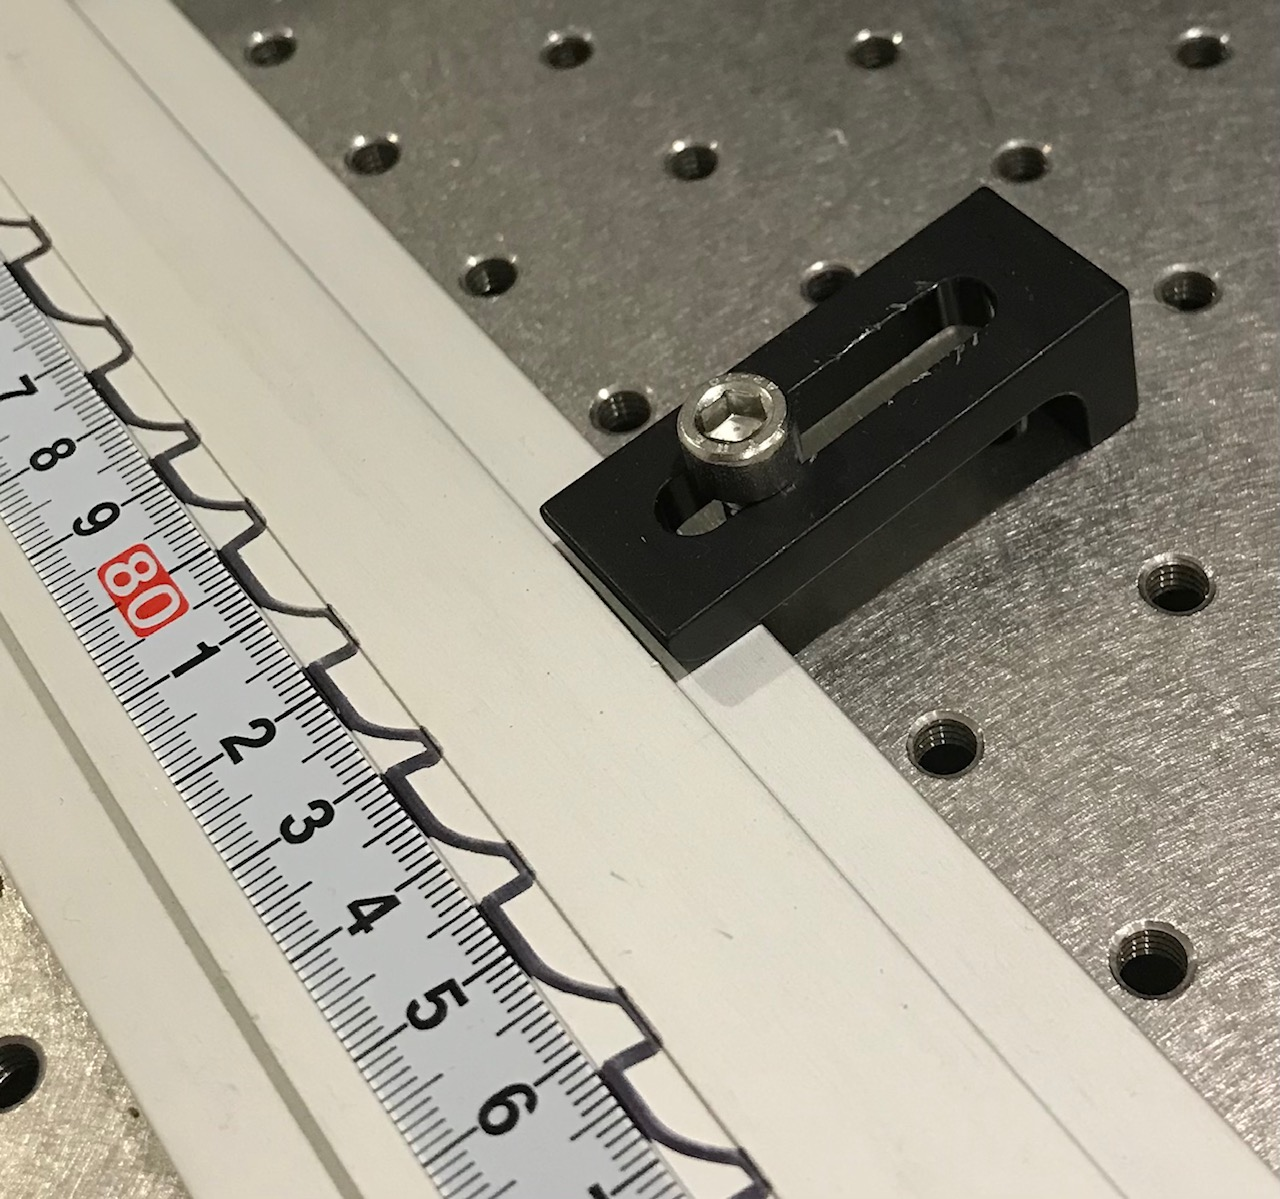
\includegraphics[width=1.25in]{figures/clamping_rail.jpg}
		\captionsetup{width=0.95\textwidth}
		\caption{Basic assembly.
		\\
		1-2. The black post holders mount to the rail carriages via a short cap screw. Place the rail carriages on the rail - unscrew the screws on the side almost all the way, then tighten just enough to slide smoothly.
		\\
		3. Use the red cylindrical lens tool to turn the retaining ring, which secures lenses in lens holders. `SM2' refers to two inch, `SM1' to one inch optics and associated accessories (shown is SM1).
		\\
		4. Clamps can be used to hold down the rail (use in a position where you won't obstruct sliding carriages).}
		\label{fig:post}
	\end{figure}
	
	
	
	%%%%%%%%%%%%%%%%%%%%%%%%%%%%%%%%%%%%%%%%%%%%%%%%%%%%%%%%%%%%%%%%%%%%%%%
	\section{Working with the laser pointer}
	%%%%%%%%%%%%%%%%%%%%%%%%%%%%%%%%%%%%%%%%%%%%%%%%%%%%%%%%%%%%%%%%%%%%%%%
	
	The following image shows how to set up a laser pointer on an adjustable tip/tilt mount. 
	Note how the pointer is mounted to a base located off the rail. 
	The laser pointer is held in an adjustable (tip/tilt) mount.
	The adjustment screws of the tip/tilt mount should face backwards, away from the beam exit.
	

	\begin{figure}[h]
		\center
		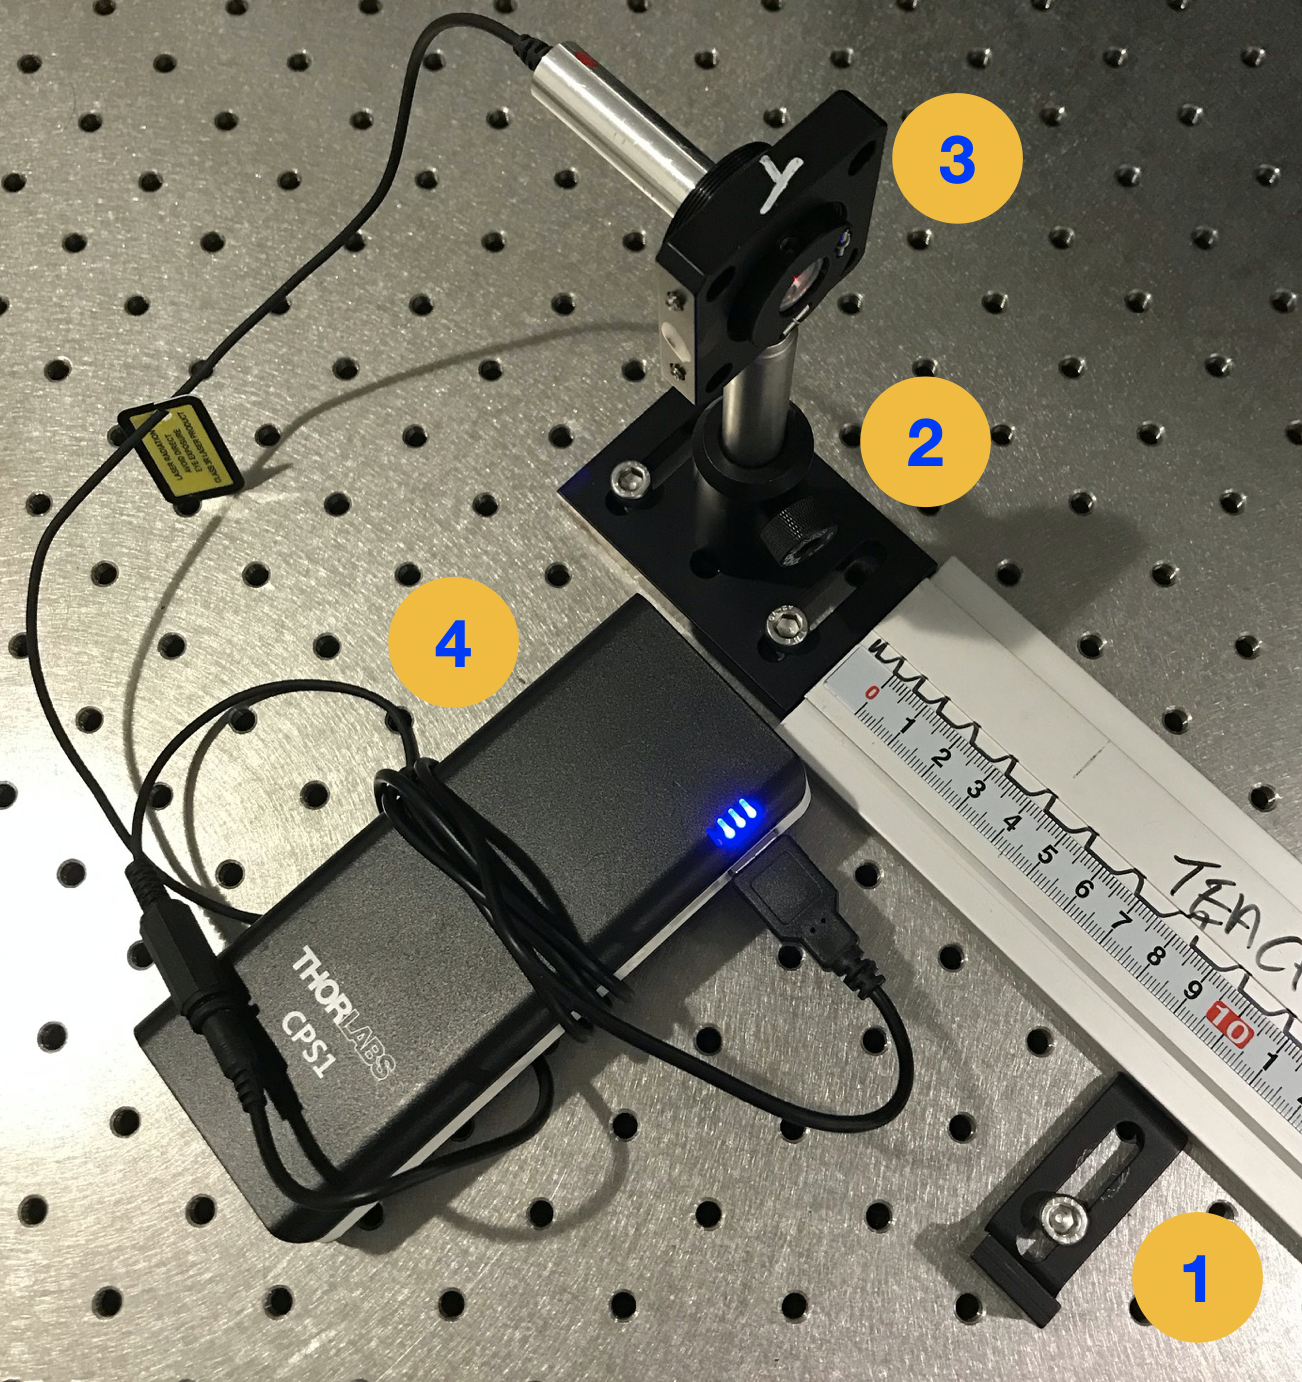
\includegraphics[width=2.17in]{figures/laser_diode.png}
		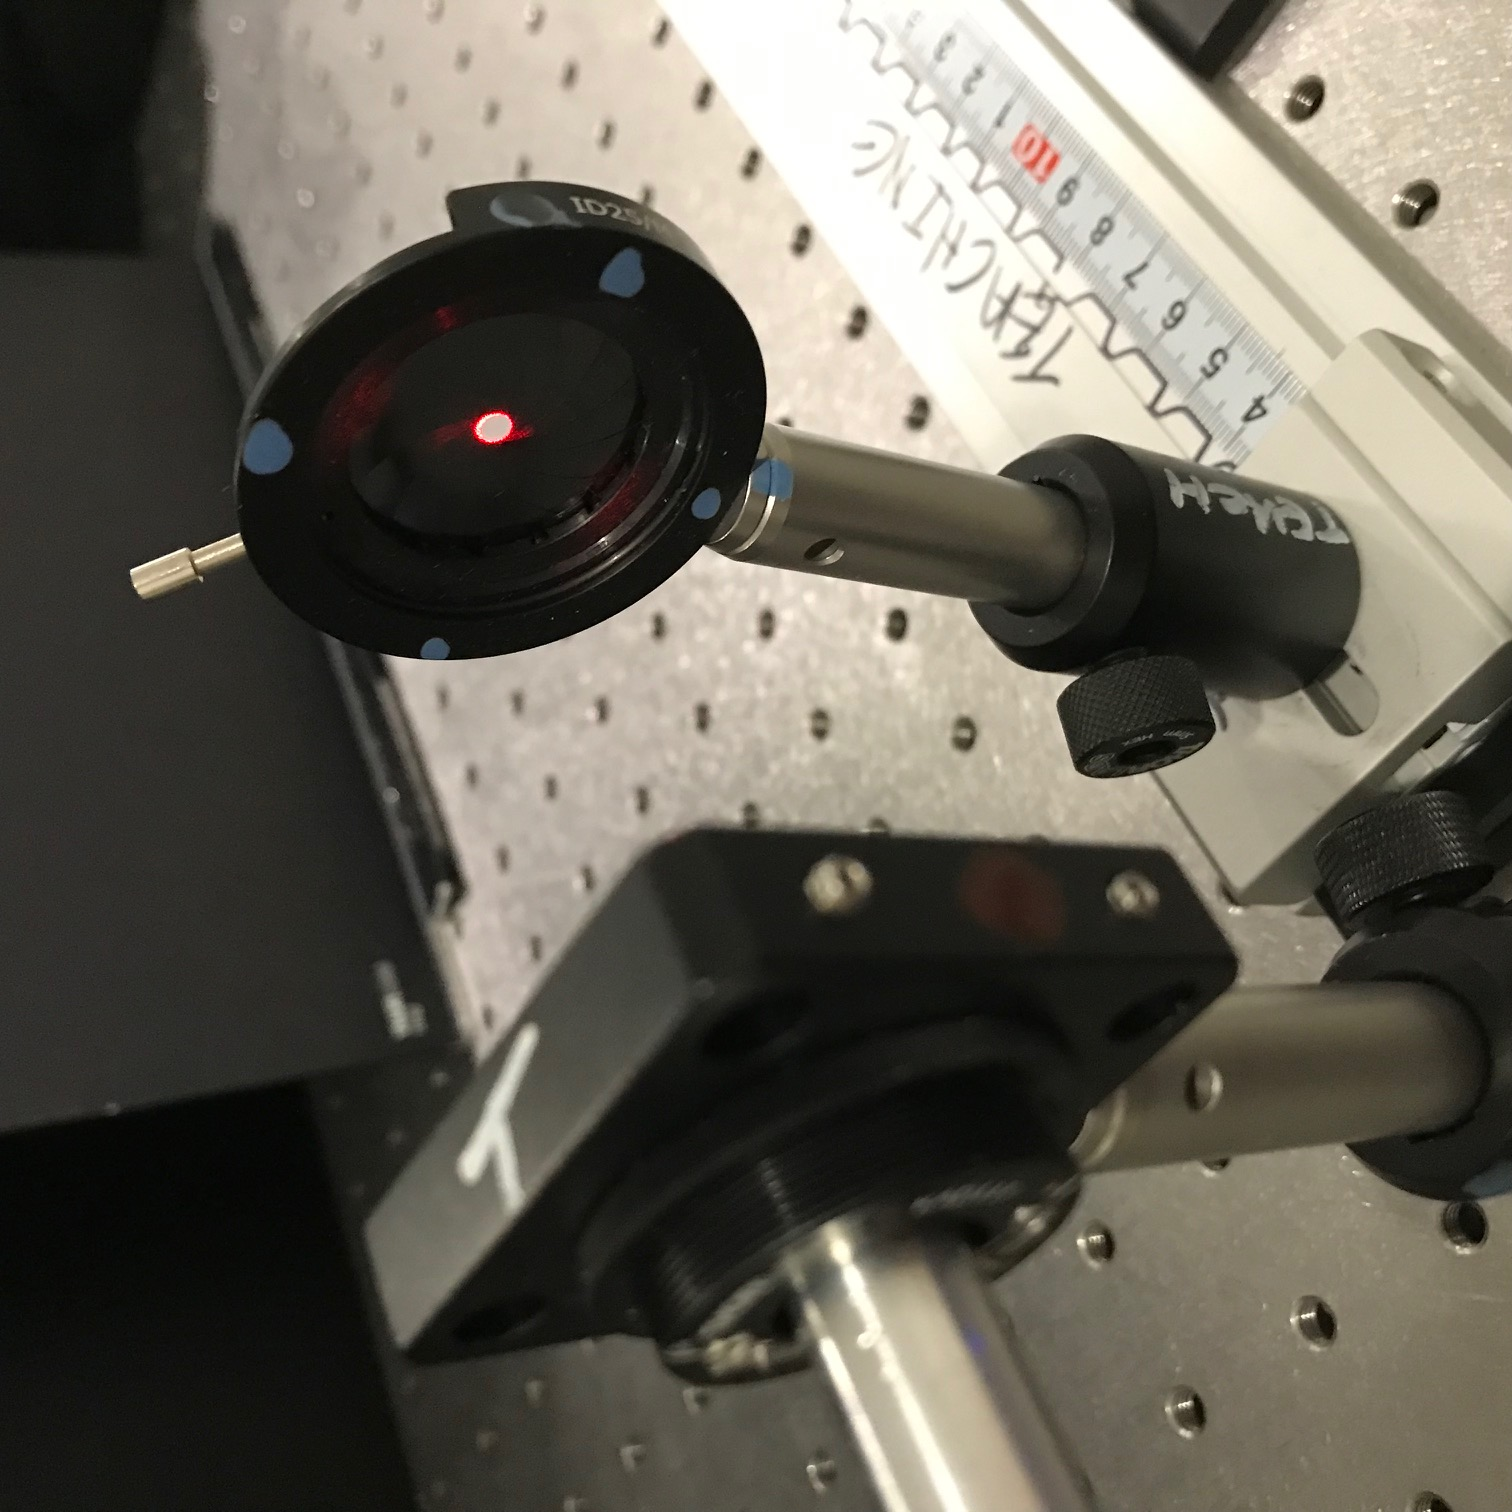
\includegraphics[width=2.3in]{figures/laser_diode_iris.jpg}
		\captionsetup{width=0.9\textwidth}
		\caption{Assembly of the laser diode and iris. \\
		Left: \\
		1. Stop the rail from moving by pushing clamps against it. \\
		2. Use a rectangular for lateral translation and push the rail against it. \\
		3. Mount the laser in the tip/tilt mount protruding minimally (using the set screw), so that it sits close to the rotational axis of the mount (important to keep changing the angle of the beam independent of changing the position). \\
		4. Plug the diode into a USB power source (can be computer too). \\
		Right: \\
		The semi-open iris indicates alignment as you slide it down the rail to the far position.}
		\label{fig:post}
	\end{figure}
	
	

	\end{document}
	